\chapter{Draft}

\section{RQ1. Com que frequência \textit{breaking changes} surgem nos pacotes clientes?}
\label{sec:rq1}

\subsection{Motivação}
\label{mot:rq1}

O \Gls{NPM} contém mais de 12 bilhões de downloads semanais e ultrapassa os 48 bilhões por mês\footnote{https://api.npmjs.org/downloads/point/last-month}. Estes pacotes são usados por milhões de pessoas e projetos por todo o mundo. Entretanto, uma simples \textit{release} que contenha um erro pode afetar uma quantidade imensa de pacotes. Isso se deve ao fato dos pacotes dependerem uns dos outros, direta ou indiretamente. Para evitar as \textit{breaking changes}, o \Gls{NPM} utiliza \textit{strings} de versionamento baseadas no \Gls{SemVer} para especificar as versões dos provedores. O versionamento permite que um provedor publique uma \textit{release} que contenha \textit{breaking changes} sem afetar os clientes das versões prévias.

Entretanto, nem sempre o desenvolvedor é capaz de distinguir se suas alterações são \textit{breaking} ou \textit{non-breaking changes} \cite{noregrets2018}, ou, muitas vezes, as \textit{breaking changes} são introduzidas sem que o programador perceba. Por exemplo, a \textit{release optipng@0.2.0} introduziu uma \textit{breaking change}: a \gls{API} \textit{OptiPng.getBinaryPath} foi renomada para \textit{OptiPng.getBinPath}. Porém, a \gls{API} foi renomeada por engano e a \textit{release} errônea foi publicada em uma versão \textit{minor}, fazendo com que todos os clientes que tinham acesso àquela \gls{API} não a tivesse mais. Assim, o código \ref{cod:bc:optipng} executa normalmente com o \textit{optipng@0.1.1}, mas ao atualizar para o \textit{optipng@0.2.0}, este código sofre uma \textit{breaking change} -- o que não deveria acontecer com uma \textit{release minor}  -- conforme mostra a Figura \ref{fig:bc_optipng} (a).

\begin{lstlisting}[style=Javascript, label=cod:bc:optipng, caption={Código que sofre \textit{breaking change} do \textit{optipng}}]
var OptiPng = require('optipng');
var cb = {apply: () => {}};
OptiPng.getBinaryPath(cb);
\end{lstlisting}

Apesar de ser um erro facilmente detectável, este foi consertado somente 34 dias após a \textit{release} errônea. E esta correção foi realizada em um \textit{commit}\footnote{https://github.com/papandreou/node-optipng/commit/a155f2b078224be18367847bbcbd3df3c379deea} no qual o desenvolvedor informou no comentário que a renomeação da \gls{API} ocorreu por engano, conforme a Figura \ref{fig:bc_optipng} (b), quando o desenvolvedor desfez a renomeação.

\begin{figure}
    \centering
    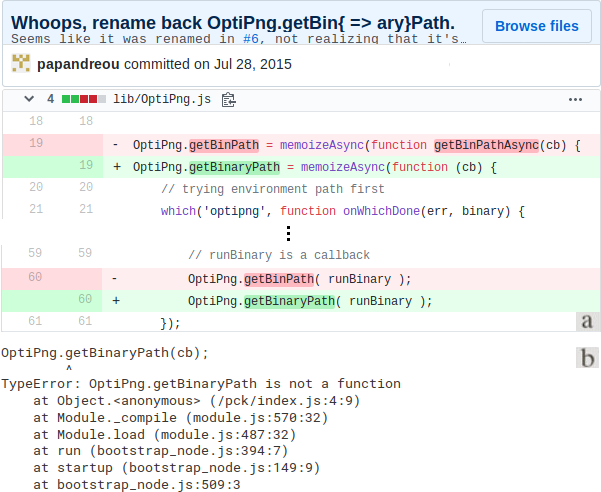
\includegraphics[scale=0.65]{figuras/bc_optipng.png}
    \caption{\textit{a}: \textit{stack trace} da \textit{breaking change}. \textit{b}: \textit{commit} que corrigiu a \textit{breaking change}}
    \label{fig:bc_optipng}
\end{figure}{}

Para responder esta RQ, será utilizado uma base de dados com os nomes de todos os pacotes do \Gls{NPM} até jun/2017. Há nesta base de dados \textit{366,629} nomes de pacotes. A quantidade de amostras para o estudo será de \textit{385} pacotes, com base em um cálculo amostral\footnote{https://pt.surveymonkey.com/mp/sample-size-calculator/} com 95\% de confiança e 5\% de margem de erro. Dos \textit{366K} de pacotes, a amostra de \textit{385} será recuperada sorteando um número no intervalo \textit{0-366,629}. Do pacote sorteado será recuperado o seu \textit{package.json} e verificado se o pacote cumpre quatro requisitos: possuir mais de 1 dependente --  se não houver dependentes, não há possibilidades do pacote sofrer \textit{breaking changes}; possuir pelo menos a última \textit{release} com \textit{script} de teste não vazio e diferente do \textit{script} padrão de teste do \gls{NPM}: \textit{Error: no test specified}; possuir a \textit{url} do repositório do pacote; e o repositório do pacote precisa existir -- será esperado de uma requisição \Gls{HTTP} para o repositório o código \textit{200} indicando sua existência. A Figura \ref{fig:package_json} exemplifica as informações pertinentes no \textit{package.json} do pacote \textit{raven@0.1.0}\footnote{http://registry.npmjs.org/raven}.

\begin{figure}
    \centering
    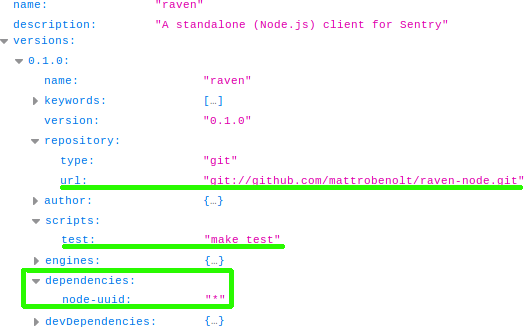
\includegraphics[scale=0.7]{figuras/package_json.png}
    \caption{Informações que serão recuperadas do \textit{package.json} para validar um pacote}
    \label{fig:package_json}
\end{figure}{}

%pacotes sorteados serão
Dos testes realizados para esta RQ serão analisados três pontos: 1) quantas vezes cada provedor publica uma \textit{release} que contém \textit{breaking changes}; 2) em qual nível da \textit{string} de versionamento as \textit{breaking changes} são tipicamente introduzidas, de acordo com o \Gls{SemVer}; 3) qual o percentual de clientes que atualizam para uma versão com \textit{breaking changes}.

\subsection{Approach}
\label{apr:rq1}

%\Gls{NPM}.
Um \textit{stack trace} contém as informações sobre as subrotinas de um programa. É utilizado para certos tipos de \textit{debugs}, nos quais eles auxiliam a visualizar e rastrear um determinado evento/erro. Quando os comandos \textit{npm install} e \textit{npm test} resultam em erro, o \Gls{NPM} mostra o erro e todas as chamadas de função, incluindo as invocações para os provedores. A Figura \ref{fig:trace} mostra um exemplo genérico de um \textit{stack trace} exibido pelo \Gls{NPM} após a ocorrência de um erro. Nesta Figura, no topo do \textit{stack trace} contém a mensagem e o tipo do erro que interrompeu a execução. Nas linhas abaixo, há cada chamada de função e seu respectivo arquivo, com a linha e a coluna que se encontra esta função. Com todos estes dados, o \textit{stack trace} auxilia no rastreamento de cada erro.

\begin{figure}
    \centering
    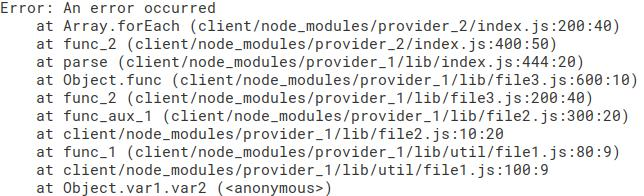
\includegraphics[scale=0.7]{figuras/stack_trace.jpeg}
    \caption{Generic stack-trace}
    \label{fig:trace}
\end{figure}{}

O \textit{stack trace} é a base da analise de um erro. A primeira etapa da análise de um erro é diferenciar entre um erro que foi causado pelo próprio pacote cliente, no qual não houve influência de nenhum provedor, e um erro que foi causado por algum dos provedores. Esta análise foi realizada de duas maneiras diferentes.

A primeira maneira foi verificar no \textit{stack trace} por chamadas de função para os provedores. Quando não há chamada para os provedores no \textit{stack trace}, provavelmente o erro não se trata de uma \textit{breaking change}. Então, a falha pode estar apenas no código do cliente. Para confirmar isto, foi procurado no \textit{GitHub} do cliente pelos próximos \textit{commits} após a data da \textit{release} no qual o desenvolvedor tenta consertar algum erro. Se sim, o código do cliente foi alterado para verificar se estas modificações realmente refletem a correção do erro. Entretanto, alguns tipos de erros já indicam exatamente em qual local o erro aconteceu. São os \textit{SyntaxError} e \textit{ReferenceError}, no qual já se sabe em qual local o erro se manifesta e o seu real motivo. O Código \ref{cod:syntax:error} mostra um exemplo deste tipo de erro. Ou seja, este tipo de erro indica que o código escrito pelo desenvolvedor está sintaticamente errado e apenas se manifesta pois o desenvolvedor escreveu o código erroneamente.

\begin{lstlisting}[style=Javascript, label=cod:syntax:error, caption={Código com um \textit{Reference Error}}]
const a = 0 = 0;
\end{lstlisting}

%evidência
A segunda maneira é quando o erro indicava a presença de \textit{breaking changes} através de chamadas para os provedores no \textit{stack trace}. Entretanto, as chamadas para \textit{frameworks} de teste, como o \textit{Mocha, Instanbul, Jasmine} entre outros, ou automatizadores de tarefas, o \textit{Grunt} por exemplo, não evidenciam inicialmente a presença de \textit{breaking changes} uma vez que eles apenas iniciam a execução do pacote e deveriam estar ali. Porém, não foi descartados a hipótese de apresentarem \textit{breaking changes}. O melhor local para se confirmar a existência da \textit{breaking change} é no \textit{GitHub} e várias técnicas foram utilizadas para recuperar as informações necessárias. A primeira foi procurar nos arquivos registros de alterações, os \textit{CHANGELOG.md} ou \textit{HISTORY.md}. Uma das informações mais relevantes nesta pesquisa são as descrições de \textit{breaking changes}. Por exemplo, a versão \textit{5.0.0} do pacote \textit{Mocha} contém uma \textit{breaking change} que foi documentada no \textit{CHANGELOG.md}\footnote{https://github.com/mochajs/mocha/blob/master/CHANGELOG.md\#500--2018-01-17} de acordo com a Figura \ref{fig:bc_documentation} (a). Outro tipo de documentação equivalente são as \textit{releases-notes}, como pode ser visualizado na Figura \ref{fig:bc_documentation} (b) como o pacote \textit{npm-wpxml2md} documentou \textit{breaking changes} nas \textit{releases-notes}. Um detalhe importante é que as chamadas para \textit{frameworks} de teste, como o \textit{Mocha, Instanbul, Jasmine} entre outros, não evidenciam diretamente -- a princípio -- a presença de \textit{breaking changes}.

\begin{figure}
    \centering
    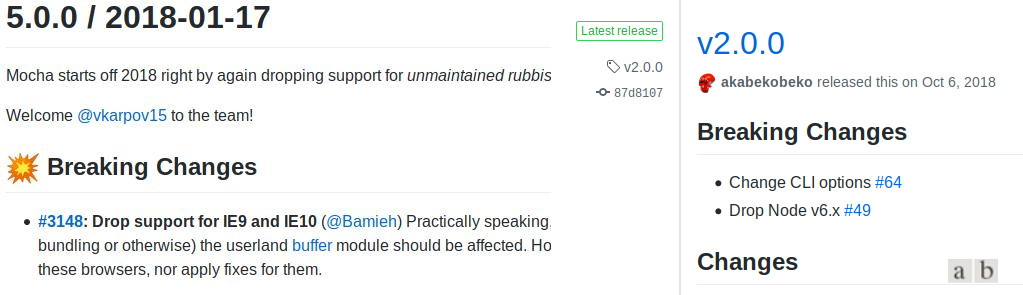
\includegraphics[scale=0.45]{figuras/bc_documentation.jpeg}
    \caption{Breaking Change documentation in CHANGELOG and release-notes}
    \label{fig:bc_documentation}
\end{figure}{}

Entretanto, apenas 46\% dos repositórios contêm algum dos dois registros. Assim, uma alternativa foi verificar nas \textit{issues} dos repositórios. Nestas, muitas informações foram encontradas.

Um ponto que foi muito importante é a instalação de versões prévias e sucessivas dos provedores. Com isso, foi possível testar a partir de qual versão o erro foi introduzido e consertado. Também, alguns outros recursos foram utilizados, tais como, o uso da ferramenta \textit{npm-diff}\footnote{https://github.com/danielventurini/npm-diff}, que provê os \textit{diff} do código entre duas \textit{releases} de um determinado pacote.

A Figura \ref{fig:step_analyze} exemplifica as técnicas utilizadas para responder esta questão de pesquisa.

\begin{figure}
    \centering
    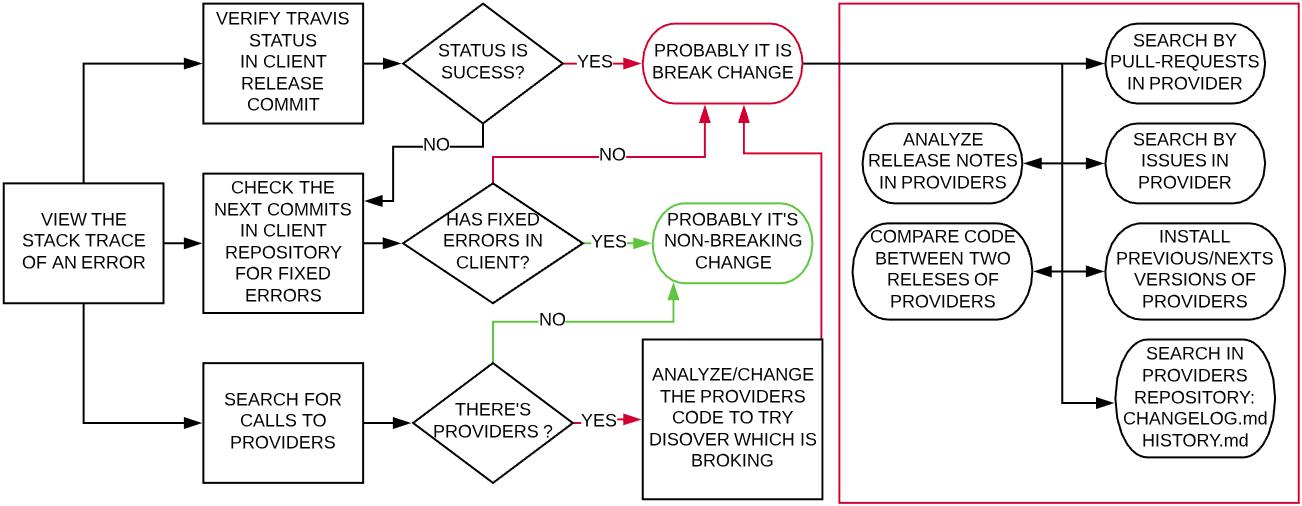
\includegraphics[scale=0.35]{figuras/step_analyze.jpeg}
    \caption{Steps to analyze an error}
    \label{fig:step_analyze}
\end{figure}

%Vale ressaltar que alguns sistemas integrados ao \textit{GitHub} auxiliaram na investigação. Esses sistemas são o \textit{Travis, Jenkins, Codeship, CicleCI} etc. Eles colaboraram ...
Vale ressaltar que alguns sistemas integrados ao \textit{GitHub} auxiliaram na investigação. Esses sistemas são o \textit{Travis, Jenkins, Codeship, CicleCI} etc. Eles foram usados da seguinte maneira: se o \textit{commit} da \textit{release} teve sucesso na execução \textit{npm install} e \textit{npm test} e, ao executá-los nesta pesquisa resultou em erro, indica que há uma \textit{breaking change}. Outro detalhe importante se refere aos pactes que utilizavam algum tipo de sistemas terceiros como o \textit{MySql, CouchDB, Redis} etc. Então, quando foi gerado um erro pela falta de um destes, fez-se a habilitação destes e o pacote foi re-executado.

Então, para todas as \textit{releases} analisadas manualmente, foi salvo as seguintes informações:

\begin{enumerate}
    \item Em que local o erro foi documentado: \textit{issue, changelog, pull-request} etc;
    \item Quem consertou o erro: cliente ou providor;
    \item Em qual nível do \textit{SEMVER} o erro foi reparado;
    \item Quanto tempo o erro levou até ser corrigido; e
    \item Por quantas \textit{releases} o erro persistiu.
\end{enumerate}{}

\subsection{Findings}
\label{fin:rq1}
Ao todo, foi executado um total de 405 pacotes. Entretanto, em 21 pacotes não foi possível executar o comando \textit{npm test} para nenhuma de suas versões. Isso porque estes pacotes apresentaram algum tipo de erro que impossibilitou a execução do teste. Destes 21 pacotes, 76\% (16) não possuía algum dos arquivo para os testes. Também, 19\% (4) haviam listados alguns dos arquivos necessários para o teste no arquivo \textit{.gitignore}, impossibilitando a execução dos testes, uma vez que estes arquivos não foram adicionados ao \textit{Github}. Por fim, um pacote foi considerado como um \textit{toy package}, ou seja, não era um projeto real, apenas um repositório no qual o desenvolvedor, provavelmente, criou para testar o \gls{NPM}. Então, todos estes pacotes foram substituídos por outros 21 pacotes. Desta maneira, a pesquisa foi realizada com um total de 385 pacotes.

\subsubsection{De todos os pacotes, 11\% foram impactados por \textit{breaking changes}}


\subsubsection{De todos os pacotes afetados, 13\% apresentaram mais de uma \textit{breaking change}}

%---------------------------------------------------%
\section{RQ2. Quais são os problemas no pacote provedor que causam \textit{breaking change}?}
\label{sec:rq2}

\subsection{Motivation}
\label{mot:rq2}

Uma pesquisa realizada por \citeonline{uncovered} mostrou que, dos 373 pacotes \textit{Javascript} utilizados, os que não possuíam \textit{scripts} de testes eram: 22\% da base estudada; 40\% dos pacotes clientes; e 3\% dos pacotes servidores. Além disso, nem sempre os casos de testes cobriam 100\% do pacote. O fato de haver pouca quantidade de casos de teste, juntamente com a dinâmica do \textit{Node.js}, corroboram para que seus códigos possam apresentar comportamentos inesperados. Por exemplo, considere o seguinte caso no qual é tentado realizar um acesso a uma posição inexistente de um vetor no Código \ref{cod:wrong:access} em três linguagens diferentes.

\begin{lstlisting}[style=javascript, label=cod:wrong:access, caption={Acesso inválido à posição de memória}, numbers=none]
// Java
int vet[] = new int[10];
vet[14] = 0;

// Python
vet = []
vet[14] = 0

// Node.js
vet = []
vet[14] = 10
\end{lstlisting}

No código escrito em \textit{Java}, um erro será gerado em tempo de compilação. Já no código em \textit{Python}, uma exceção será gerada em tempo de execução. Entretanto, apenas no código \textit{Javascript} nenhum erro/aviso é gerado e o usuário não será informado sobre esse comportamento, uma vez que esse é um comportamento esperado do \textit{Node.js}. Isso porque o interpretador \textit{Node.js} aloca 14 posições na memória nas quais 13 dessas possuem o valor \textit{undefined} e a décima quarta, o valor \textit{10}. Assim, a dinâmica do \textit{Node.js} dificulta a busca por erros, uma vez que um caso errôneo é tratado pelo interpretador como um caso normal.

%Para responder essa questão de pesquisa, será analisado caso a caso dos erros e as \textit{breaking changes} serão categorizadas 

Para responder essa RQ será analisado dois pontos: 1) quais são as categorias de erros que causam \textit{breaking changes}; e 2) quantificar essas categorias pela quantidade de \textit{releases} afetadas e pelo número de clientes que sofreram com esta determinada categoria. Como a análise manual irá descobrir o real motivo de uma \textit{breaking change}, elas poderão ser classificadas e quantificadas de uma forma mais clara. Assim sendo, dimensionar as categorias ajudará os desenvolvedores a atentar-se para estas categorias e tentar evitá-las.

\subsection{Approach}
\label{apr:rq2}

O objetivo da análise manual era descobrir o real motivo que originou um erro e agrupa-los por suas similaridades. Isso, porque o \textit{stack trace} sempre apresenta o erro de uma maneira genérica. Então, as vezes, a mensagem de erro pode induzir a interpretação errônea do real motivo que originou a falha. Por exemplo, a Figura \ref{fig:error_category} mostra dois casos no qual uma função foi renomeada pelo provedor. Entretanto, previamente não está claro o real motivo dos erros.

\begin{figure}[!h]
    \centering
    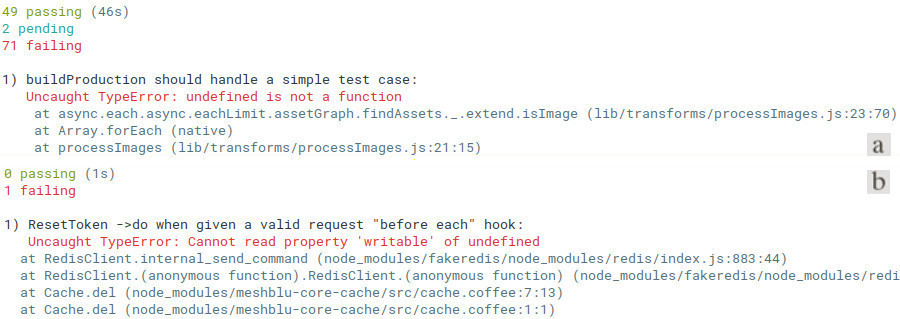
\includegraphics[scale=0.5]{figuras/error_category.jpeg}
    \caption{Dois erros causados pelo mesmo motivo mas com \textit{stack trace} diferentes}
    \label{fig:error_category}
\end{figure}

A mensagem do primeiro erro (a) deixa claro que se trata de uma invocação a uma função inexistente. Assim, somente pela mensagem do \textit{stack trace} é possível deduzir que uma função foi renomeada no provedor. Já no segundo erro (b), o \textit{stack trace} não indica que se trata de uma função renomeada. Somente após uma análise deste caso é que foi possível concluir que o erro se trata de uma função que não existia. Por isso se fez necessário a análise manual para reconhecer os reais motivos de cada caso de erro.

Após descobrir que um erro diz respeito à alteração de \gls{API}, por exemplo, uma categoria chamada \textit{Função Renomeada} será criada e as demais \textit{breaking changes} que possuem características comuns a esta também serão categorizadas como \textit{Função Renomeada}. Assim será possível quantificar cada uma das categorias. E mesmo processo será realizado para as demais \textit{breaking changes}, sempre visando criar categorias da maneira mais genérica que agrupe os erros semelhantes.

\subsection{Findings}
\label{fin:rq2}

%---------------------------------------------------%
\section{RQ3. Como os pacotes clientes se recuperam das breaking change?}
\label{sec:rq3}

\subsection{Motivation}
\label{mot:rq3}

Uma vez que uma \textit{breaking change} é introduzida o provedor deve se recuperar desta. Isso se faz necessário pois, no ecossistema \gls{NPM}, no qual centenas de milhares de pacotes estão conectados, uma simples \textit{release} com erro pode ocasionar na quebra de muitos clientes. Isso ocorreu com um pacote chamado \textit{left-pad}\footnote{https://blog.npmjs.org/post/141577284765/kik-left-pad-and-npm}. Esse foi removido do \textit{NPM} por seu desenvolvedor e impactou milhares de pacotes em apenas 2.5 horas incluindo \textit{babel}\footnote{https://github.com/babel/babel} e \textit{atom}\footnote{https://github.com/atom/atom}.

As vezes, o provedor deixa dar a manutenção por algum motivo. Então, os clientes recebem esta responsabilidade. No caso do \textit{left-pad} o provedor nunca publicou uma nova \textit{release} e, para que todos os pacotes continuassem a executar normalmente, um dos clientes publicou um pacote com o mesmo nome e mesmo código.

No entanto, como os provedores evoluem independentemente dos clientes, erros e vulnerabilidades são difíceis de rastrear e corrigir nos clientes. Mesmo quando as vulnerabilidades podem ser corrigidas com a atualização para uma versão mais recente do provedor, pode haver incompatibilidades de \textit{API} -- entre outras incompatibilidades -- com os clientes que deve ser resolvido manualmente \cite{Foo:2018:ESC:3236024.3275535}. Assim, o cliente dificilmente irá conseguir ter sucesso quanto a resolução do erro no provedor. Então, uma alternativa para o cliente é mudar de provedor buscando por um que atenda as necessidades que não fora atendidas pelo provedor prévio.

Para responder a questão de pesquisa final, foi analisado três pontos: 1) o que aconteceu para que o provedor não pudesse consertar o erro; 2) como o cliente consertou o erro: no seu código ou notificando o provedor através de \textit{issues} e \textit{pull-requests}; 3) quantas vezes o cliente teve que realizar a correção dado que o provedor não a fez. Todas as informações sobre esta questão de pesquisa estão nos \textit{commits}, \textit{issues}, \textit{pull-requests}, \textit{changelogs} e \textit{releases-notes} dos repositórios do cliente e do provedor.

\subsection{Approach}
\label{apr:rq3}

Uma vez que os clientes se recuperaram de um erro, há duas maneiras para se obter informações sobre esta recuperação. A primeira maneira é quando o provedor corrige seu código e o cliente apenas atualiza sua \textit{string} de versionamento no \textit{package.json}, se precisar. Para o provedor consertar o erro, deve haver uma \textit{issue} no seu repositório. A segunda maneira é quando o próprio cliente conserta o código. Neste caso, o cliente pode corrigir o código do provedor e realizar um \textit{pull-request}. Também, o cliente pode alterar apenas o seu código para que execute normalmente com a \textit{release} errônea do provedor. Há casos também no qual nem o cliente nem o provedor faz nada para consertar o erro.

Todas as informações sobre esta questão de pesquisa foram recuperadas do \textit{GitHub}. As informações foram encontradas em \textit{CHANGELOGs, release-notes, issues} e \textit{pull-requests}. Se os \textit{CHANGELOGs} contêm informações sobre os erros consertados, geralmente, as \textit{issues} são marcadas. A partir das \textit{issues} uma grande quantidade de informações podem ser recuperadas. Pois, assim como o código de um pacote fica emaranhado com o código no restante do ecossistema ao qual ele pertence, o mesmo acontece com as \textit{issues}. Uma manifestação disso é que muitas \textit{issues} abertas em um projeto são vinculadas a \textit{issues} relacionadas, em projetos iguais ou diferentes, pois os desenvolvedores estão rastreando as causas de um problema \cite{Zhang:2018:WIL:3242887.3242891}. De maneira análoga, os \textit{pull-requests} que são relacionados ao mesmo problema também são marcados. Todas estas informações corroboram para descobrir como a \textit{breaking change} foi tratada/consertada e quem -- cliente ou provedor -- a consertou, caso tenha sido consertada.

Os \textit{commits} são alternativas para as \textit{issues} quando a busca se dá no repositório do cliente. Sobre os \textit{commits}, mensagens do tipo \textit{update dependencies, fix dependencies, fix errors} etc. sugerem que algum provedor foi atualizado para consertar algum erro ou um erro foi consertado diretamente no código do cliente. Esta informações é muito importante, uma vez que o provedor corrigiu a \textit{breaking change} e o cliente apenas o atualizou. Assim, as mensagens dos \textit{commits} auxiliaram para descobrir os reais motivos da atualização -- ou retrocesso da versão.

\subsection{Findings}
\label{d_fin:rq3}
